\chapter {Analyse spectrale}

%-------------------------------------
\section{Introduction}
%-------------------------------------

L'analyse spectrale est l'étude des valeurs propres et des vecteurs propres d'une matrice carrée. \\
Les valeurs propres\index{valeur propre}
d'une matrice carrée $A (n\times n)$ sont les $n$ solutions dans $\mathbb{C}$ de l'équation caractéristique
$$det(\lambda I-A) = 0$$
Du point de vue de l'algèbre linéaire, cela signifie que le noyau de $\lambda I-A$ contient des vecteurs non nuls, appelés vecteurs propres\index{vecteurs!propres} associés à $\lambda$.
Donc, si $x\neq 0$ est un vecteur propre  de $A$ associé à la valeur propre $\lambda$,
on a $Ax=\lambda x$.

Le calcul des $n$ solutions de l'équation caractéristique est coûteux dès que $n>2$ et le théorème d'Abel montre qu'on ne peut 
espérer la résoudre par des radicaux
dès que $n>4$. On recherchera donc des méthodes itératives qui permettent d'approcher ces racines et non de les calculer explicitement car, à la différence des méthodes de résolution de systèmes linéaires vues dans le chapitre 2, la convergence sera ici asymptotique. En fait, les méthodes qui seront présentées pour le calcul des valeurs propres sont utilisées pour extraire les racines d'un polynôme en passant par la matrice compagne :  
$$\dsum_{i=0}^{n-1}a_it^i+t^n = 0$$
est le polynôme caractéristique\index{polynôme caractéristique}
de la matrice compagne\index{matrice!compagne}
$$A =
\left (
\begin{array}{llll}
0 & \cdots &  &-a_0\\
1  &\ddots && -a_1\\
0 & & 0 &\vdots\\
0 & & 1 & -a_{n-1}
\end{array}
\right )
$$ 

%-------------------------------------------------
\section{Intérêts de l'analyse spectrale} %-------
%-------------------------------------------------

Considérons par exemple un système d'équations différentielles ordinaires : \index{système!différentiel}\\
Trouver les fonctions $v(t)$ et $w(t)$, pour $t\in \mathbb{R}^+$, telles que :
\begin{eqnarray*}
\frac{dv}{dt}& =& 4v - 5w\\[.25pc]
\frac{dw}{dt}& =& 2v - 3w
\end{eqnarray*}
avec comme conditions initiales $v(0)=8,w(0)=5$.
Ce système peut être mis sous la forme vectorielle
\begin{equation}\label{eqvec}
\frac{du}{dt}=Au
\end{equation}
avec : $$u(t)=\begin{pmatrix}v(t)\\w(t)\end {pmatrix},u(0)=\begin{pmatrix}8\\5\end {pmatrix},A=\begin{pmatrix}4\quad -5\\2\quad -3\end {pmatrix}$$
Sachant que la solution de l'équation $x'=ax$ en dimension 1 est $x(t)=x_0e^{at}$, qui diverge si $a>0$ et se stabilise asymptotiquement à zéro si $a<0$, on cherchera des solutions particulières de la forme 
$$
\left \{
\begin{array}{cc}
v(t) =& \tilde{v}e^{\lambda t}\\
w(t) =& \tilde{w}e^{\lambda t}
\end{array}
\right .
$$ 
En remplaçant dans (\ref{eqvec}), on voit que 
$$
u(t)=e^{\lambda t}\begin{pmatrix}
                            \tilde{v}\\ \tilde{w}
                  \end{pmatrix}
    \Rightarrow \frac{du}{dt}=\lambda e^{\lambda t}
                  \begin{pmatrix}
                             \tilde{v}\\ \tilde{w}
                  \end{pmatrix}=Au(t)
$$
d'où 
$$
A\begin{pmatrix}\tilde{v}\\\tilde{w}\end{pmatrix}
=\lambda\begin{pmatrix}\tilde{v}\\\tilde{w}\end{pmatrix}
$$
et $\lambda$ doit donc être une valeur propre de $A$ associée au vecteur propre $\begin{pmatrix}\tilde{v}\\\tilde{w}\end {pmatrix}$. Dans le cas présent, on calcule aisément les éléments propres de $A$ :
\begin{align*}
\lambda_1=-1 & \Rightarrow \begin{pmatrix}\tilde{v_1}\\\tilde{w_1}\end {pmatrix}=\begin{pmatrix}1\\1\end {pmatrix} \Rightarrow u^1(t)=\begin{pmatrix}e^{-t}\\e^{-t}\end {pmatrix}\\
\lambda_1=2 & \Rightarrow \begin{pmatrix}\tilde{v_2}\\\tilde{w_2}\end {pmatrix}=\begin{pmatrix}5\\2\end {pmatrix} \Rightarrow u^2(t)=\begin{pmatrix}5e^{2t}\\2e^{2t}\end {pmatrix}
\end{align*}
La linéarité du système implique que toute combinaison linéaire des solutions particulières $u^1,u^2$ est solution de l'équation différentielle. La solution générale s'écrit donc :
$$u(t)=\alpha u^1(t)+\beta u^2(t)$$
où $\alpha=3$ et $\beta=1$ sont déterminées par les conditions initiales.

%------------------------------------
\section{Résultats généraux} %-------
%-------------------------------------

On donnera ici quelques propriétés d'intérêt surtout pratique concernant les valeurs propres et les vecteurs propres de certaines matrices. Les démonstrations sont omises, et on se référera à l'ouvrage de G. Strang \cite{SG:88}, pour plus de détails.

Une matrice carrée $A$ de dimension $n$ à coefficients complexes ou réels possède $n$ valeurs 
propres non nécessairement distinctes dans $\mathbb{C}$. L'ensemble de ces valeurs propres est 
le \textbf{spectre} \index{spectre d'une matrice} de $A$, noté $\mathrm{sp}(A)$, et le nombre de fois où apparaît une 
valeur propre $\lambda$ dans ce spectre est appelé sa 
\textbf{multiplicité}.\index{valeur propre!multiplicité}
Le \textbf{rayon spectral},\index{rayon spectral} noté $\rho(A)$, est le plus grand module des valeurs propres de $A$. La somme des valeurs propres est égale à la \textbf{trace} 
\index{matrice!trace} de la matrice :
$$
\dsum_{i=1}^n\lambda_i=\dsum_{i=1}^na_{ii}
$$
et on en déduit donc que si une matrice réelle possède une valeur propre complexe, son conjugué est aussi valeur propre. De même, le produit des valeurs propres est égal au \textbf{déterminant}
 \index{matrice!déterminant} de 
$A$ :
$$
\prod_{i=1}^n\lambda_i=det(A)
$$
Donc $A$ non singulière $\Leftrightarrow$ $0\notin \mathrm{sp}(A)$.

\textbf{Attention !} Il n'est pas possible en général d'obtenir valeurs et vecteurs propres de la somme ou du produit de deux matrices dont on connaît le spectre, mais certains cas particuliers où les vecteurs propres sont les mêmes permettent de conclure :
\begin{itemize}
	\item si $\lambda$ est valeur propre de $A$,  $\lambda^k$ est valeur propre de $A^k$ (en particulier, si $A$ est inversible, $\lambda^{-1}$ est valeur propre de l'inverse)
	\item  si $\lambda$ est valeur propre de $A$, $\lambda+\alpha$ est valeur propre de $A+\alpha I$.
\end{itemize}
\vskip 10pt
Si $\lambda$ est une valeur propre de $A$, le système $(A-\lambda I)x=0$ possède des solutions non nulles appelées \textbf{vecteurs propres} \index{vecteurs!propres}
de $A$ associés à $\lambda$. On appelle \textbf{sous-espace propre} \index{sous-espace!propre}
associé à une valeur propre $\lambda$ le noyau de $A-\lambda I$. Sa dimension est donc au moins égale à 1.

Lorsque les valeurs propres sont distinctes, les vecteurs propres sont linéairement indépendants. L'implication réciproque est fausse, on pensera au cas de la matrice identité pour s'en 
convaincre.

Si les $n$ vecteurs propres $x_i,1\leq i\leq n$ peuvent être choisis linéairement indépendants, ils forment une matrice $X=\left [ x_i\right ]$ non singulière, et on a :
$$
X^{-1}AX=\Lambda=\mathrm{diag}\{\lambda_1\cdots\lambda_n\}
$$
En effet, $AX$ est la matrice dont les colonnes sont les vecteurs $Ax_i=\lambda x_i$ qui est bien égale à $X\Lambda$. On dit dans ce cas que {\gr $A$ est diagonalisable}
\index{matrice!diagonalisable}
et cette propriété ne peut s'écrire qu'avec la matrice des vecteurs propres. 
Elle caractérise le fait que $X$ a pour colonnes des vecteurs propres et que ces vecteurs 
propres sont linéairement indépendants.


Observation : il existe des matrices qui ne sont pas diagonalisables (on les appelle 
matrices \textbf{défectives}\index{matrice!défective}). Elles satisfont aux deux conditions 
suivantes :
\begin{itemize}
	\item il existe des valeurs propres multiples
	\item  la dimension du sous-espace propre associé est strictement inférieure à la multiplicité de la valeur propre.
\end{itemize}
Attention, le seul fait de l'existence de valeurs propres multiples ne suffit pas à impliquer que la matrice soit défective ({\it cf.} la matrice identité par exemple).
Un exemple typique de matrice défective est $A=\begin{pmatrix} 0\quad 1\\0\quad 0\end{pmatrix}$, qui possède la valeur propre double 0. Les vecteurs propres sont de la forme $x=\begin{pmatrix}\alpha\\0\end{pmatrix}$, ils engendrent donc un sous-espace de dimension 1. $A$ n'est donc pas diagonalisable.

Dans certains cas, il est relativement facile d'inférer sur la valeur ou la nature des valeurs propres d'une matrice $A$:
\begin{itemize}
	\item si $A$ est diagonale, les valeurs propres sont les éléments diagonaux
	\item si $A$ est triangulaire, les valeurs propres sont également les éléments diagonaux
	%\item si $A$ est non singulière, les valeurs propres sont toutes différentes de 0
	\item si $A$ est orthogonale, les valeurs propres ont pour module 1 et il est possible de choisir une base de vecteurs propres orthonormés
	\item si $A$ est symétrique, ses valeurs propres sont réelles. Les vecteurs propres associés à des valeurs propres distinctes sont 
alors orthogonaux. On a $\|A\|_2=\rho(A)$.
\end{itemize}
Le dernier point implique en particulier que toute matrice réelle symétrique est diagonalisable par une matrice orthogonale : $\Lambda=Q^\top AQ$,où $Q$ est formée par $n$ vecteurs propres orthonormés. On a alors la \textbf{factorisation spectrale} \index{factorisation!spectrale}
d'une matrice symétrique réelle :
$$A=Q\Lambda Q^\top $$
\vskip 10pt
En résumé de ce qui précède :
{\gr 
\begin{itemize}
	\item l'inversibilité est liée aux valeurs propres
	\item la diagonalisabilité est liée aux vecteurs propres
\end{itemize}
}

%-------------------------------------------
\section{Similitudes}  %--------------------
%-------------------------------------------
L'objectif est encore une fois de transformer une matrice par des transformations simples en une matrice dont on connaît les valeurs propres, c'est-à-dire, une matrice triangulaire ou diagonale. Les transformations qui maintiennent le spectre d'une matrice sont des similitudes.

%-----------------------------------------------------
\subsection{Définition et propriétés} %---------------
%-----------------------------------------------------

\begin{defin}
Deux matrices carrées $A$ et $B$ sont dites \textbf{semblables} \index{matrice!semblables}
s'il existe une matrice $S$ non singulière telle que 
$$B=S^{-1}AS$$
\end{defin}
La transformation de $A$ vers $B$ est une {\gr similitude}. En l'écrivant sous la forme $AS=SB$, on retrouve une généralisation de la définition des valeurs propres et des vecteurs propres. On a d'ailleurs le résultat fondamental :
\begin{prop}
Deux matrices semblables ont les mêmes valeurs propres
\end{prop}
\textsc{Démonstration:} soit $x$ un vecteur propre de $A$ associé à la valeur propre $\lambda$. On a donc $Ax=\lambda x$, qui s'écrit $SBS^{-1}x=\lambda x$, ce qui veut dire que $\lambda$ est valeur propre de $B$ associé au vecteur propre $S^{-1}x$.\hfill$\Box$


L'intérêt de ces transformations est double : 
\begin{itemize}
	\item les valeurs propres sont inchangées
	\item en supposant les vecteurs propres linéairement indépendants, la similitude associée à la matrice $X$ dont les colonnes sont les vecteurs propres transforme $A$ en une matrice diagonale dont les éléments diagonaux sont les valeurs propres de $A$ : $X^{-1}AX = \Lambda$.
\end{itemize}

Montrons maintenant sur un exemple que deux matrices semblables représentent la même transformation linéaire sur deux bases différentes : soit $P$ la matrice de projection dans $\mathbb{R}^2$ sur la droite $L$ d'angle $\theta$ : 
$$P =
\left[
\begin{array}{cc}
\cos^2(\theta) & \cos(\theta)\sin(\theta)\\
\cos(\theta)\sin(\theta)& \sin^2(\theta)
\end{array}
\right]
=uu^\top \quad\mbox{avec}\quad u=\begin{pmatrix}\cos(\theta)\\ \sin(\theta)\end{pmatrix}
$$ 
Si on fait maintenant tourner la base canonique orthonormée d'un angle $\theta$, la projection devient maintenant une projection sur l'axe horizontal et s'écrit
$$Q =
\left[
\begin{array}{cc}
1&0\\
0&0\\
\end{array}
\right]
$$ 
Pour passer de $P$ à $Q$, on utilise la matrice de rotation d'angle $\theta$ 
$$R =
\left[
\begin{array}{cc}
\cos(\theta) & -\sin(\theta)\\
\sin(\theta)& \cos(\theta)
\end{array}
\right]
$$ 
Le changement de base se traduit par : si $x$ est le vecteur de coordonnées dans la base de départ, et $u$ le vecteur de coordonnées dans la base d'arrivée, on a 
$$x=Ru$$
Soit $y$ la projection de $x$ sur $L$ dans la base de départ, et $v$ ses coordonnées dans la base d'arrivée. Alors 
\begin{align*}
y &= Px\\
Rv&= PRu\\ \Rightarrow v&=R^{-1}PRu=Qu
\end{align*}
et donc 
$$Q=R^{-1}PR$$
et donc $P$ et $Q$ ont les mêmes valeurs propres. Comme $Q$ est diagonale, on retrouve ici le résultat connu : toute matrice de projection sur une droite dans $\mathbb{R}^2$ a pour valeurs propres 1 et 0, et pour vecteurs propres associés les colonnes de la matrice de rotation $R$, c'est-à-dire les directions de $L$ et $L^{\bot}$ respectivement.

%-----------------------------------------------------
\subsection{Théorème de Gershgorin} %-----------------
%-----------------------------------------------------
Une alternative pratique aux algorithmes de calcul approché des valeurs propres que nous décrirons plus loin est le théorème suivant qui permet de localiser les valeurs propres dans des disques, dits disques de Gershgorin, du plan complexe.

\begin{theo}[Théorème de Gershgorin]\index{théorème!de Gershgorin} 
Si on représente une matrice $A$ (ou toute matrice semblable à $A$) sous la forme $A=diag\{d_1\cdots d_n\}+F$, où $F$ est une matrice de diagonale nulle, alors le spectre de $A$ est contenu dans l'union des disques $D_i,1\leq i\leq n$ du plan complexe, tels que 
$$D_i=\left \{ z\in \mathbb{C}, |z-d_i|\leq \dsum_{j=1}^n|f_{ij}|\right \}$$
\end{theo}

\textsc{Démonstration:} soit $\lambda$ une valeur propre supposée différente des $d_i,1\leq i\leq n$. Alors $(D-\lambda I)+F$ est singulière et d'après le théorème 3.1, on a la majoration $\|(D-\lambda I)^{-1}F \|\geq 1$. Le choix de la norme $\|.\|_{\infty}$ 
fournit le résultat cherché.\hfill$\Box$

Une application intéressante de ce résultat est l'estimation des valeurs propres d'une matrice obtenue en perturbant une matrice dont on connaît le spectre.

\begin{exemple} 
$$A =
\left[
\begin{array}{ccc}
1&0.1&-0.1\\
0&2&0.4\\
-0.2&0&3\\
\end{array}
\right]
$$ 
dont les valeurs propres sont situées dans les disques suivants (Figure \ref{51})
\begin{align*}
D_1&=\left \{ z\in \mathbb{C}, |z-1|\leq 0.2\right\}\\
D_2&=\left \{ z\in \mathbb{C}, |z-2|\leq 0.4\right\}\\
D_3&=\left \{ z\in \mathbb{C}, |z-3|\leq 0.2\right\}
\end{align*}
\end{exemple}

\begin{figure}[H]
\begin{center}
	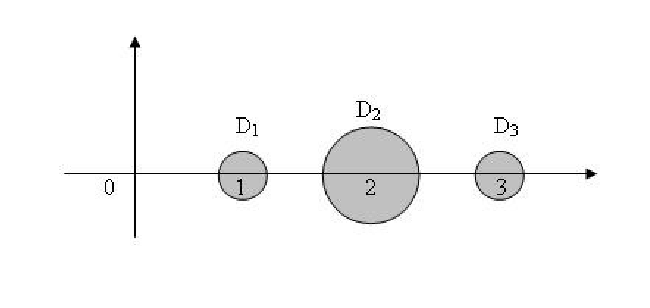
\includegraphics[width=22em]{gershgorin.eps}
\end{center}
\caption{disques de Gershgorin}
\label{51}
\end{figure}

%-----------------------------------------------------------------------------------------
\section{Calcul des valeurs propres d'une matrice symétrique : méthode de Jacobi}
%-----------------------------------------------------------------------------------------
L'intérêt principal des matrices réelles symétriques est qu'il existe une base de vecteurs propres orthonormés. On peut donc la diagonaliser par une transformation orthogonale : soient $A$ une telle matrice et $Q$ la matrice orthogonale dont les colonnes sont les vecteurs propres de $A$, alors $Q^\top AQ=diag\{\lambda_1\cdots \lambda_n\}$.

La méthode de Jacobi est une méthode d'élimination symétrique itérative utilisant des similitudes orthogonales :
\begin{itemize}
	\item la matrice transformée tend vers une matrice diagonale
	\item le produit des transformations orthogonales tend vers la matrice des vecteurs propres.
\end{itemize}

%--------------------------------------------------------
\subsection{Principe d'élimination symétrique}  %-------
%-------------------------------------------------------
Ce principe, basé sur des rotations successives, sera illustré tout d'abord sur une matrice (2$\times$2) : soit $A$ la sous-matrice (2$\times$2) symétrique 
$$
A=\begin{pmatrix}a_{pp}\quad a_{pq}\\
         a_{pq}\quad a_{qq}
   \end{pmatrix}\quad a_{pq}\neq 0.
$$
Soit $R$ la matrice de rotation d'angle $-\theta$ : 
$$
R = \begin{pmatrix}\cos\theta \quad  \sin\theta\\ 
                  -\sin\theta\quad  \cos\theta
    \end{pmatrix}.
$$
Pour éliminer l'élément $a_{pq}$ non diagonal, on détermine $\theta$ tel que 
$$
R^\top AR=\begin{pmatrix}*\quad0\\0\quad *\end{pmatrix}
$$
Le calcul donne 
$$
\mathrm{cotg}(2\theta)=\frac{a_{qq}-a_{pp}}{2a_{pq}}
$$
Considérons maintenant une matrice symétrique $n\times n$ $A$ telle que l'élément $a_{pq}$ soit non nul. La transformation orthogonale $\Omega$ telle que $A'=\Omega^\top A\Omega$, avec $a'_{pq}=a'_{qp}=0$ est :
$$
\Omega =
\left (
\begin{array}{ccccc}
1&&&&\\
&\ddots& \cos\theta & \sin\theta&\\
&&-\sin\theta & \cos\theta&\\
&&&\ddots&\\
&&&&1\\
\end{array}
\right )
\left .
\begin{array}{c}
p\\
q\\
\\
\end{array}
\right .
$$ 
On vérifie que seules les lignes et colonnes $p$ et $q$ de $A$ sont modifiées. 
En posant $c=\cos\theta$, $s=\sin\theta$, $t=\tan\theta$, la mise à jour s'écrit :
\begin{align*}
a'_{pj}&=ca_{pj}-sa_{qj},j\neq p,q\\
a'_{qj}&=ca_{qj}+sa_{pj},j\neq p,q\\
a'_{pp}&=a_{pp}-ta_{pq}\\
a'_{qq}&=a_{qq}+ta_{pq}
\end{align*}
Un choix classique pour $p$ et $q$ est celui qui permet d'éliminer l'élément non diagonal de plus grand module : $|a_{pq}|=\displaystyle\max_{i\neq j}|a_{ij}|$

%-----------------------------------
\subsection{Convergence}
%-----------------------------------
Soit $\{A_k\}$ la suite de matrices engendrée par l'algorithme en éliminant à chaque itération un élément non diagonal non nul ($A_0=A$) et son symétrique. Comme la transformation est orthogonale, la norme de Frobenius de la matrice est conservée ({\it cf} chapitre 3) : 
$$
\dsum_{i,j}a_{ij}'^2=\dsum_{i,j}a_{ij}^2
$$
Mais ce même résultat est vrai pour la matrice (2$\times$2) transformée ci-dessus. Donc :
$$a'^2_{pp}+a'^2_{qq}=a^2_{pp}+a^2_{qq}+2a_{pq}^2$$
Comme seules les lignes $p$ et $q$ sont modifiées, ces résultats impliquent que la somme des carrés des éléments diagonaux augmente strictement de la valeur $2a_{pq}^2$, et que la somme des carrés des éléments non diagonaux diminue strictement de la même quantité.\\
On démontre alors le théorème suivant :
\begin{theo}
La suite de matrices $\{A_k\}$ engendrée par la méthode de Jacobi classique converge vers une matrice diagonale contenant toutes les valeurs propres de $A$ sur la diagonale
\end{theo}
\textsc{Démonstration:} voir par exemple Ciarlet \cite{CPG:82} (voir aussi l'exercice \ref{exo54})


On peut également démontrer que, si les valeurs propres sont toutes distinctes, la suite des matrices $Q_k=\Omega_1\cdots \Omega_k$ converge vers la matrice orthogonale contenant les vecteurs propres.

\textbf{Attention !} : un élément annulé peut redevenir non nul aux itérations suivantes.

%--------------------------------------
\subsection{Observations}  %-----------
%--------------------------------------
\begin{itemize}
	\item Le tri du plus grand élément parmi $n(n-1)/2$ coûtant relativement cher, on lui préfère d'autres stratégies plus économiques (balayage cyclique ou choix avec seuil)
	\item La méthode de Jacobi présente d'excellentes performances pour des matrices pleines de faible dimension (typiquement inférieure à 100). Dans le cas général, on lui préférera la méthode QR ({\it cf.} ci-après).
\end{itemize}

%-------------------------------------------------------------------------------
\section{Calcul de certains vecteurs propres : les puissances itérées}
%-------------------------------------------------------------------------------

%-----------------------------------
\subsection{Quotient de Rayleigh}
%------------------------------------
Pour une matrice symétrique $A$, le quotient de Rayleigh\index{quotient de Rayleigh}
est le rapport défini pour tout vecteur $x\neq 0$ par :
$$\rho_A(x)=\frac{x^\top Ax}{x^\top x}$$
On vérifie immédiatement que si $x$ est vecteur propre, le quotient de Rayleigh fournit la valeur propre associée : en effet $Ax=\lambda x \Rightarrow x^\top Ax=\lambda x^\top x$.

Si $\lambda_1$ et $\lambda_n$ sont respectivement la plus petite et la plus grande valeur propre de $A$, et $x^1$,$x^n$ les vecteurs propres associés, on a également les résultats suivants :
\begin{align*}
\lambda_1&=\rho_A(x^1)=\displaystyle\min_{x\in \mathbb{R}^n}\{\rho_A(x)\}\\
\lambda_n&=\rho_A(x^n)=\displaystyle\max_{x\in \mathbb{R}^n}\{\rho_A(x)\}
\end{align*}
De plus, si les valeurs propres sont rangées dans l'ordre croissant, on a 
\begin{align*}
\lambda_i&=\displaystyle\min_{S_i}\{\displaystyle\max_{x\in S_i}\{\rho_A(x)\}\}\\
\lambda_i&=\displaystyle\max_{S_{i-1}}\{\displaystyle\min_{x\in S_{i-1}^\bot}\{\rho_A(x)\}\}
\end{align*}
où $S_i$ est un sous-espace quelconque de dimension $i$.
\vskip 10pt
Le sous-espace $S_i$ pour lequel le quotient de Rayleigh est maximum est le sous-espace propre associé aux $i$ premières valeurs propres. Le sous-espace pour lequel il est minimum est orthogonal au sous-espace propre associé aux $i-1$ premières valeurs propres. C'est donc le sous-espace engendré par les $n-i+1$ vecteurs propres associés à $\{\lambda_i\cdots\lambda_n\}$.

%-----------------------------------------------------
\subsection{Méthode des puissances itérées}  %--------
%-----------------------------------------------------

La méthode des puissances itérées permet de calculer le vecteur propre associé à la plus grande valeur propre.
Supposons $A$ symétrique de valeurs propres ordonnées selon $$|\lambda_1|\leq\cdots|\lambda_{n-1}|<|\lambda_n|$$
On considère l'itération suivante définie à partir d'un vecteur initial $q_0$ donné, tel que $\|q_0\|=1$, et $q_0$ n'est pas orthogonal à $v^n$, le vecteur propre associé à la plus grande valeur propre isolée $\lambda_n$ :
\begin{align*}
x_{k+1}&=Aq_k\\
q_{k+1}&=\frac{x_{k+1}}{\|x_{k+1}\|}
\end{align*}
Par récurrence, on montre que 
$$q_k=\frac{A^kq_0}{\|A^kq_0\|}$$
 et comme les vecteurs propres $\{v^1\cdots v^n\}$ forment une base de $\mathbb{R}^n$, on peut écrire 
 $$q_0=\dsum_{i=1}^n\alpha_iv^i,\quad\alpha_n\neq 0$$
 et 
 $$A^kq_0=\alpha_n\lambda_n^k\left (v^n+\dsum_{i=1}^{n-1}\frac{\alpha_i}{\alpha_n}\left (\frac{\lambda_i}{\lambda_n}\right )^kv^i\right )$$
 Lorsque $k\rightarrow\infty$, les rapports $\left (\frac{\lambda_i}{\lambda_n}\right )^k$ tendent vers 0 pour $i\neq n$, 
 ce qui signifie que la suite des itérés $\{q_k\}$ converge vers le vecteur propre $v^n$ ou $-v^n$. 
 On peut montrer de plus que $\|Aq_k\|$ tend vers $|\lambda_n|$ et que la convergence est linéaire de taux $\left |\frac{\lambda_{n-1}}{\lambda_n}\right |$ si $\alpha_{n-1}\neq 0$.

%--------------------------------------------------------
\subsection{Méthode des puissances inverses}  %----------
%--------------------------------------------------------
Pour les mêmes raisons, l'itération 
\begin{align*}
Ax_{k+1}&=q_k\\
q_{k+1}&=\frac{x_{k+1}}{\|x_{k+1}\|}
\end{align*}
avec $\|q_0\|=1$, et $q_0$ n'est pas orthogonal à $v^1$, converge vers la direction du vecteur propre associé à la plus 
petite valeur propre en module. On remarquera le coût de calcul en $O(n^2)$.

\subsection{Remarques}
\begin{enumerate}
	\item Accélération par \textbf{décalage} : la matrice $A+\alpha I$ a les mêmes vecteurs propres que $A$ et ses valeurs propres sont décalées de la quantité $\alpha$. La méthode des puissances itérées inverses converge d'autant plus vite que les rapports $\left|\frac{\lambda_1}{\lambda_2}\right|^k$ tendent rapidement vers 0. On a donc intérêt à ce que $\lambda_1$ soit le plus proche possible de 0, et de plus, la méthode sera d'autant plus rapide que l'écart entre les deux plus petites valeurs propres se creuse. La technique du décalage consiste donc à remplacer $A$ par $A+\alpha I$, avec $\alpha\approx -\lambda_1$. Plus l'estimation de $\lambda_1$ sera précise, plus la convergence sera rapide. Toutefois, il faut que $\alpha\neq -\lambda_1$ pour éviter que la matrice ne devienne singulière
	\item Technique de \textbf{déflation} : la méthode des puissances itérées peut être étendue pour permettre le calcul de toutes les valeurs propres d'une matrice symétrique. Supposons en effet calculée la plus grande valeur propre $\lambda_n$ ainsi qu'un vecteur propre associé $v^n$. Soit $P_n$ la la matrice de projection orthogonale sur l'hyperplan $(v^n)^\bot$. La matrice $P_nA$ possède les mêmes vecteurs propres que $A$ et les mêmes valeurs propres à l'exception de $\lambda_n$ qui est remplacée par 0. L'application de la méthode des puissances itérées à $P_nA$ permettra donc de calculer la deuxième plus grande valeur propre de $A$. Cette technique, dite de déflation, permet théoriquement de calculer toutes les valeurs propres de $A$. Elle est toutefois numériquement instable sans précautions, et on lui préférera généralement la méthode des puissances groupées présentée ci-après.
\end{enumerate}

%--------------------------------------------------------
\section{Puissances groupées et méthode QR}  %-----------
%--------------------------------------------------------

On peut généraliser la méthode des puissances itérées à des itérations dites groupées, permettant d'identifier les vecteurs propres associés aux $p$ plus grandes valeurs propres
en valeur absolue. A chaque itération, on applique la transformation $A$ à chacun des vecteurs orthonormés, et on orthogonalise (par Gram-Schmidt ou Householder, {\it cf.} chapitre 4) le système résultant.

\subsection{Itération des puissances itérées}

Soit $\{q_1^{(k)}\cdots q_p^{(k)}\}$ un système de $p$ vecteurs orthonormés obtenu à l'itération $k$
\begin{itemize}
	\item construire le système $\{Aq_1^{(k)}\cdots Aq_p^{(k)}\}$
	\item calculer les quotients de Rayleigh : $\lambda_i={q^{(k)}_i}^\top Aq_i^{(k)},\quad 1\leq i\leq p$
	\item tester la convergence : $\displaystyle\max_{1\leq i\leq p} \|Aq_i^{(k)}-\lambda_i q_i^{(k)} \|<Tol$
	\item orthogonaliser $\{Aq_1^{(k)}\cdots Aq_p^{(k)}\} \rightarrow \{q_1^{(k+1)}\cdots q_p^{(k+1)}\}$
\end{itemize}

%-----------------------------------
\subsection{Méthode QR}  %----------
%-----------------------------------

La méthode QR correspond au cas $p=n$ : soit $Q_k$ la matrice ($n\times n$) dont les colonnes sont les vecteurs orthogonaux $q_i^{(k)}$ et soit $A_k=Q_k^\top AQ_k$ la représentation de $A$ sur la base des $\{q_i^{(k)}\}$. On peut écrire alors (Gram-Schmidt) : 
$$
AQ_k=Q_{k+1}R_{k+1}
$$ 
où $R_{k+1}$ est triangulaire supérieure. Et ainsi 
\begin{align*}
A_k&=Q_k^\top Q_{k+1}R_{k+1}=QR_{k+1}\\
A_{k+1}&=Q_{k+1}^\top AQ_{k+1}=R_{k+1}Q_k^\top Q_{k+1}=R_{k+1}Q
\end{align*}
En résumé, $Q$ est la matrice orthogonale qui permet de triangulariser $A_k$ et on écrit $A_{k+1}$ en inversant le produit $QR$. La méthode QR prend alors la forme particulièrement simple suivante :
\begin{itemize}
	\item $A_0=A$
	\item $A_k=Q_kR_k$ (par Gram-Schmidt par exemple)
	\item $A_{k+1}=R_kQ_k$
	\item test sur le plus grand élément non diagonal
\end{itemize}
\vskip 10pt
Observons que $A_{k+1}=Q^\top A_kQ$, ce qui implique que les matrices sont toutes semblables et que la suite des matrices  $Q$ converge vers la matrice des vecteurs propres. La matrice $A_k$ converge vers une matrice diagonale où les valeurs propres sont rangées dans l'ordre décroissant (Figure \ref{52}). 

\begin{figure}[htpb]
\begin{center}
	\includegraphics[width=22em]{QR.eps}
\end{center}
\caption{diagonalisation d'une matrice 8$\times$8 par QR d'après \cite{LGT:89}}
\label{52}
\end{figure}

Les performances sont considérablement améliorées si on intègre deux modifications :
\begin{itemize}
	\item {\gr décalage} de la matrice en prenant comme approximation de la plus petite valeur propre l'élément ($n\times n$) de $A_k$
	\item transformation préalable de $A$ en une matrice {\gr tridiagonale}. Les matrices $A_k$ restent tridiagonales et l'orthogonalisation s'effectue en $O(n)$ flops.
\end{itemize}

%----------------------------
\section{Exercices} %--------
%----------------------------
\begin{exo}[Diagonalisation]\rm
Soit les matrices 
$$
\bm 
1 & 1 \\
0 & 2 
\em
, 
\bm 
1 & 0 \\
1 & 2 
\em
,
\bm 
1 & 1 \\
0 & 1 
\em
,
\bm 
1 & 1 \\
1 & 0 
\em
,
\bm 
1 & 2 \\
2 & 4 
\em,
$$

$$
%\bm 
%\cos\theta & -\sin\theta \\
%\sin\theta & \cos\theta 
%\em,
\bm 
0 & 1 & 0 \\
1 & 0 & 1 \\
0 & 1 & 0
\em
,
\bm 
11 & -5 & 5 \\
-5 & 3 & -3 \\
5 & -3 & 3
\em
$$

Pour chacune de ces matrices, répondre aux questions suivantes :
\begin{itemize}
\item Polynôme caractéristique ?
\item Spectre et rayon spectral ?
\item Multiplicité algébrique des valeurs propres ?
\item Sous-espaces propres ?
\item Multiplicité géométrique des valeurs propres ?
\item La matrice est-elle diagonalisable ?  Si oui, la diagonaliser.
%\item Donner une interprétation de l'application linéaire associée à la matrice.
\end{itemize}
\end{exo}

\begin{exo}[Interprétation géométrique des éléments propres]\rm

Que peut-on dire de la diagonalisabilité, des valeurs propres et des vecteurs propres
\begin{itemize}
\item  d'une homothétie ?
\item d'un projecteur ?
\item d'une rotation?
\end{itemize}
\end{exo}

\begin{exo}[Applications de la diagonalisation]\rm


\begin{enumerate}
\item 


Soit $A=\bm 
1 & 1 \\
0 & 2 
\em$.
Exprimer  la matrice $A^k$.

\item 
Soit la suite de Fibonacci $1$, $1$, $2$, $3$, $5$, $8$, $13$, ... définie par :
\begin{align*}
u_0&=u_1=1,\\
u_{k}&=u_{k-1}+u_{k-2}, \quad k\geq 2.
\end{align*}
En posant $X_k=\bm u_{k+1} \\ u_k \em$, déterminer la matrice $A$ telle que $X_k=A X_{k-1} $ puis en déduire la limite de $F_k=\frac{u_{k+1}}{u_k}$ quand $k$ tend vers l'infini.


\item Soit les suites récurrentes linéaires simultanées suivantes :
$$
\left\lbrace\begin{array}{l}
u_0=v_0=0,w_0=1\\
u_{n+1}=11u_n-5v_n+5w_n\\
v_{n+1}=-5u_n+3v_n-3w_n\\
w_{n+1}=5u_n-3v_n+3w_n
\end{array}\right.
$$
Exprimer $u_n,v_n,w_n$ en fonction de $n$, pour $n\geq 0$. 
\item

Résoudre le système différentiel suivant (variable $t$, inconnues $x(t), y(t), z(t)$ à valeurs réelles)
$$
\left\lbrace\begin{array}{l}
x'(t)=y(t)\\
y'(t)=x(t)+z(t)\\
z'(t)=y(t)
\end{array}\right.
$$

\end{enumerate}
\end{exo}


\begin{exo}\rm
1.--- Soit $a$ et $b$ deux réels et $D$ une matrice carrée. Montrer que si
$\lambda$ est valeur propre de $D$, alors $a\lambda+b$ est une valeur
propre de $aD+b\mbb I$, o\`u $\mbb I$ est la matrice identité.

2.--- Soit $D$ la matrice carrée tridiagonale définie par
\begin{eqnarray*}
&&d_{ii}=0,\quad i=1,\ldots,n\\
&&d_{i,i+1}=d_{i+1,i}=1,\quad i=1,\ldots,n-1\\
&&d_{ij}=0,\quad\mbox{ailleurs}.
\end{eqnarray*}
Pour $j=1,\ldots,n$, soit $\mbf x^{(j)}$ le vecteur de $\mbb R^n$ dont
la $i$--ème composante est
$$
x_i^{(j)}=\sin 2i\frac{j\pi}{n+1}.
$$
Montrer que $\mbf x^{(j)}$ est un vecteur propre de $D$ associée à la
valeur propre 
$$
\lambda_j=2\cos 2\frac{j\pi}{n+1}.
$$

3.--- En déduire les vecteurs propres et les valeurs propres de la
matrice $4\times 4$ suivante
$$
A=\left[\begin{array}{rrrr}
	2 & -1 &  0 &  0\\
       -1 &  2 & -1 &  0\\
        0 & -1 &  2 & -1\\
        0 &  0 & -1 &  2
        \end{array}
  \right]
$$
\end{exo}


 

%\begin{exo}[Suite de Fibonacci]\rm
%On considère la suite $1$, $1$, $2$, $3$, $5$, $8$, $13$, ...
%définie par
%\begin{eqnarray*}
%&&u_0=1,\ \ \ u_1=1,\\
%&&u_k=u_{k-1}+u_{k-2},\quad k\ge 2.
%\end{eqnarray*}
%Calculer une valeur approchée de $\theta_k=u_{k+1}/u_k$, en utilisant les puissances
%itérées.  
%\end{exo}


 

\begin{exo}\rm
Soit $a$ et $b$ deux vecteurs non colinéaires de $\mbb R^n$, $\norme{a}=\norme{b}=1$. Déterminer
les vecteurs propres et les valeurs propres de la matrice $n\times n$
$$
A=aa^\top +bb^\top .
$$
\end{exo}

 

\begin{exo}[Convergence de la méthode de Jacobi]\label{exo54}\rm
Soit $A'=A+E$, la somme de deux matrices symétriques. Les valeurs propres
de ces trois matrices sont notées
$$
\lambda'_1\le \lambda'_2\le\cdots\le\lambda'_n,\quad
\lambda_1\le \lambda_2\le\cdots\le\lambda_n,\quad
\mu_1\le\mu_2\le\cdots\le\mu_n.
$$

1.--- Montrer les propriétés suivantes pour tout $i=1,\ldots,n$
\begin{description}
\item[(i)] $\lambda_i+\mu_1\le\lambda'_i\le\lambda_i+\mu_n$
\item[(ii)] $|\lambda'_i-\lambda_i|\le \parallel E\parallel$, quelle que soit 
la norme matricielle $\parallel\cdot\parallel$.
\end{description}

2.--- Soit $E^{(k)}=A^{(k)}-\mathrm{diag}(a_{ii}^{(k)})$, o\`u les
$A^{(k)}$ sont les matrices engendrées par la méthode de Jacobi.
En utilisant la norme $\parallel E\parallel_F=(\mbox{trace}(E^\top E))^{1/2}$,
montrer que $E^{(k)}$ tend vers la matrice nulle, lorsque 
$k\longmapsto \infty$.

3.--- En déduire le théorème de convergence de la méthode de Jacobi, i.e.
\begin{description}
\item[(i)] $a_{ij}^{(k)}\longrightarrow 0$, pour $i\ne j$
\item[(ii)] chaque $a_{ii}^{(k)}\longrightarrow \lambda_i$, o\`u $\lambda_i$
est une valeur propre de $A$. 
\end{description}
\end{exo}

\begin{exo}\rm
Supposons calculée la plus grande valeur propre $\lambda_n$ d'une 
matrice symétrique $A$ et le vecteur propre associé $v_n$.

1.--- Quelle est la matrice $P_n$ de projection orthogonale sur 
$v_n^\perp$.

2.--- Montrer que $P_nA$ a les m\^emes vecteurs propres que $A$, à
l'exception de $v_n$. Quelles sont les valeurs propres de $P_nA$.
En déduire une première méthode de calcul des plus grandes valeurs 
propres de $A$.
\end{exo}


\begin{exo}[Examen février 2002]\rm
 Chaque année, une proportion $a$ de clermontois quitte Clermont-Ferrand pour s'installer 
dans le Puy de Dôme (hors Clermont-Ferrand), une proportion $b$ de non clermontois
du Puy de Dôme s'installe à Clermont-Ferrand ($0\le a,b\le 1$). On pose $x_0$ le nombre
de Clermontois, et $y_0$ le nombre de non clermontois (du Puy de Dôme), en cette année.
 Au bout de $k$ années, ces nombres vaudront $x_k$ et $y_k$. On suppose qu'il n'y a pas
de flux migratoire du Puy de Dôme vers l'extérieur, et vice versa.

\begin{enumerate}
 \item Calculer $x_k$ et $y_k$ en fonction de $a$, $b$, $x_0$ et $y_0$.
\item  A quelle condition sur $a$ et $b$ existe-t-il une limite pour $x_k$ et
$y_k$ lorsque $k\rightarrow+\infty$? Que vaut cette limite?
\item Application numérique: calculer cette limite en fonction de $x_0$ et $y_0$ lorsque
$a=0.1$ et $b=0.2$.
\end{enumerate}
\end{exo}





